\chapter{Introduction}

\section{Defining lines, circles and the set of constructable points}
First we need to define what construction using a ruler and compass means.
We will use $\mathbb{C}$ as plane of drawing and $\mathcal{M} \subset \mathbb{C}$ as the set of constructed points.

\begin{definition}[Line]
    \label{def:line}
    \lean{line}
    \leanok
    A line $l$ through two points $x,y\in\mathbb{C}$ for $x\ne y$ is defined by the set: $$l:=\{\lambda x+(1-\lambda)y\mid\lambda\in\mathbb{R}\}.$$
\end{definition}

\begin{definition}[parallel]
    \label{def:parallel}
    \lean{parallel}
    \leanok
    \uses{def:line}
    Two lines $l_1$ and $l_2$ are parallel if they have the same slope, i.e. $\exists c\in\C: l_1 = \{x + r \mid x\in l_2\}$.
\end{definition}

\begin{lemma}[Parallel defined by basis]
    \label{lem:parallel_by_basis}
    \lean{parallel_basis}
    \leanok
    \uses{def:line, def:parallel}
   If the basis of two lines is is moved by the same amound, i.e $l_1.z_1 - l_2.z_1 = l_1.z_2- l_2.z_2$, then they are parallel.
\end{lemma}
\begin{proof}
    \uses{def:line, def:parallel}
    We have to lines $l_1, l_2$ with basis $z_1, z_2$ and $l_1.z_1 - l_2.z_1 = l_1.z_2- l_2.z_2$. To show that ther are parallel we have to show that $$\exists r: l_1 = \{z + r \mid z\in l_2\}.$$
    To make it esiar to read we define $a := l_1.z_1$, $b:= l_1.z_2$, $x:= l_2.z_1$ and $y:= l_2.z_2$.\\
    We use $z:= a - b$ by unfollding the definition we net to show $\exists t: t \cdot a +(1-t)\cdot b=z \iff \exists s :s \cdot x+(1-s)y+(a-x)=z$.\\
    $\Rightarrow:$ Claim $s = \frac{t(a-b)}{x-y}$ is a solution.\\
    \begin{proof}
    \begin{align*}
        && z &= s \cdot x+(1-s)y+(a-x)&&| z:= t\cdot a+(1-t)\cdot b\\
        &\Leftrightarrow & t\cdot a+(1-t)\cdot b  &= s \cdot x+(1-s)y+(a-x)\\
        &\Leftrightarrow & t\cdot a-t\cdot b +b &= s \cdot x-s\cdot y + y+(a-x)&& | -y\\
        &\Leftrightarrow & t\cdot a-t\cdot b + b-y  &= s \cdot x-s\cdot y+(a-x)-y&&| a-x =b-y\\
        &\Leftrightarrow & t\cdot a-t\cdot b  &= s \cdot x+s\cdot y\\
        &\Leftrightarrow & t(a-b)  &= s(x-y)&&|s:= \frac{t(a-b)}{x-y}\\
        &\Leftrightarrow & t(a-b)  &= \frac{t(a-b)}{x-y}(x-y)\\
        &\Leftrightarrow & t(a-b)  &= t(a-b)
    \end{align*}
    \end{proof}
    $\Leftarrow:$ Claim $t = \frac{s(x-y)}{a-b}$ is a solution.
    \begin{proof}
    \begin{align*}
        && t\cdot a+(1-t)b &= z&&| z:= s \cdot x+(1-s)y+(a-x)\\
        &\Leftrightarrow& t\cdot a-t\cdot b+b &= s \cdot x-s\cdot y+y+(a-x)&&|-y;a-x =b-y\\
        &\Leftrightarrow& t(a-b) &= s(x-y)&&|t:= \frac{s(x-y)}{a-b}\\
        &\Leftrightarrow& \frac{s(x-y)}{a-b}(a-b) &= s(x-y)
    \end{align*}
    \end{proof}
\end{proof}

\begin{definition}[Circle]
    \label{def:circle}
    \lean{circle}
    \leanok
    A circle $c$ with center $z\in\mathbb{C}$ and radius $r\in\mathbb{R}_{\ge 0}$ is defined by the set: $$c:=\{z\in\mathbb{C} \mid\|z-c\|=r\}.$$
\end{definition}

\begin{definition}[Set of lines]
    \label{def:set_of_lines}
    \lean{L}
    \leanok
    \uses{def:line}
    $\mathcal{L(M)}$ is the set of all real straight lines $l$, with $| l\cap \mathcal{M} |\ge 2$. As set this is:
    \begin{equation*}
        \mathcal{L(M)} := \{l \mid l = \{x,y\} \text{ with }x,y \in \mathcal{M} \land x \neq y\}.
    \end{equation*}
\end{definition}

\begin{definition}[Set of circles]
    \label{def:set_of_circles}
    \lean{C}
    \leanok
    \uses{def:circle}
    $\mathcal{C(M)}$ is the set of all circles in $\mathbb{C}$, with center in $\mathcal{M}$ and radius of $\mathcal{C}$ which is the distence of two points in $\mathcal{M}$. As equation this is:
    $$\mathcal{C(M)}:=\{c\mid c = \langle c, \dist r_1 r_2 \rangle \text{ with } c,r_1,r_2\in M\}.$$
\end{definition}

\begin{definition}[Ruels to construct a point]
    \label{def:rules_to_constructed_a_point}
    \lean{ill,ilc,icc,ICL_M}
    \leanok
    \uses{def:set_of_lines, def:set_of_circles}
    We define operations that can be used to construct new points.
    \begin{enumerate}
        \item $(ILL)$ is the cut of two lines in $\mathcal{L(M)}$.
        \item $(ILC)$ is the cut of a line in $\mathcal{L(M)}$ and a circle in $\mathcal{C(M)}$.
        \item $(ICC)$ is the cut of two circles in $\mathcal{C(M)}$.
    \end{enumerate}
    $ICL(\mathcal{M})$ is the set $\mathcal{M}$ combiened of all points that can be constructed using the operations $(ILL)$, $(ILC)$ and $(ICC)$ and $\mathcal{M}$.
\end{definition}

\begin{definition}[Set of constructable points]
    \label{def:set_of_constructable_points}
    \lean{M_I,M_inf}
    \leanok
    \uses{def:rules_to_constructed_a_point}
    We define inductively the chain
    \begin{equation*}
        \mathcal{M}_0 \subseteq \mathcal{M}_1 \subseteq \mathcal{M}_2 \subseteq \dots
    \end{equation*}
    with $\mathcal{M}_0 = \mathcal{M}$ and $\mathcal{M}_{n+1} = ZL(\mathcal{M}_n)$.\newline
    And call $\mathcal{M}_{\infty} = \bigcup_{n \in \mathbb{N}} \mathcal{M}_n$ the set of all constructable points.
\end{definition}

\section[The set of constructable points]{The Set $M_{\infty}$}\label{set_of_constructable_points}
When we want to work with the set of constructable points we need some basic lemmas.

\begin{lemma}[$\mathcal{M}\subseteq ICL(\mathcal{M})$]
    \label{lem:M_in_ICL_M}
    \lean{M_in_ICL_M}
    \leanok
    \uses{def:rules_to_constructed_a_point}
    Every set $M$ is in include in the constructable points of $M$, i.e.
    \[M \subseteq ICL(M)\]
\end{lemma}
\begin{proof}
    Folws from the definition of $ICL(M)$.
\end{proof}

\begin{lemma}[$\mathcal{M}_i$ Monoton]
    \label{lem:M_i_monoton}
    \lean{M_I_Monotone,M_I_Monotone_elm,M_I_Monotone', M_I_Monotone_elm'}
    \leanok
    \uses{def:set_of_constructable_points}
    The set $\mathcal{M}_i$ is monoton, i.e. $$\mathcal{M}_i \subseteq \mathcal{M}_{i+1}.$$
    This can be generalised to $$\forall m :\forall n\le m : \mathcal{M}_n \subseteq \mathcal{M}_m.$$
\end{lemma}
\begin{proof}
    Follows from the definition of $\mathcal{M}_i$.
\end{proof}

\begin{lemma}[$\mathcal{M}$ in $\mathcal{M}_i$]
    \label{lem:M_in_Mi}
    \lean{M_in_M_I }
    \leanok
    \uses{def:set_of_constructable_points}
    The set $\mathcal{M}$ is in $\mathcal{M}_i$, i.e. $$\mathcal{M} \subseteq \mathcal{M}_i.$$
\end{lemma}
\begin{proof}
    \uses{lem:M_i_monoton}
    Combeing the fact that $\mathcal{M}_0 = \mathcal{M}$ \ref{def:set_of_constructable_points} and the monotonity of $\mathcal{M}_i$ \ref{lem:M_i_monoton} we get the result.
\end{proof}

\begin{lemma}[$\mathcal{M}_i$ in $\mathcal{M}_{\infty}$]
    \label{lem:M_i_in_M_inf}
    \lean{M_I_in_M_inf,M_I_in_M_inf_elm}
    \leanok
    \uses{def:set_of_constructable_points}
    The set $\mathcal{M}_i$ is in $\mathcal{M}_{\infty}$, i.e. $$\mathcal{M}_i \subseteq \mathcal{M}_{\infty}.$$
\end{lemma}
\begin{proof}
    Follows from the definition of $\mathcal{M}_{\infty}$.
\end{proof}

\begin{lemma}[$\mathcal{m}$ in $\mathcal{M}_{\infty}$]
    \label{lem:M_in_M_inf}
    \lean{M_M_inf}
    \leanok
    \uses{def:set_of_constructable_points}
    The set $\mathcal{M}$ is in $\mathcal{M}_{\infty}$.
\end{lemma}
\begin{proof}
    \uses{lem:M_i_in_M_inf, lem:M_in_Mi}
    Combeing $\mathcal{M} \subseteq \mathcal{M}_i$ \ref{lem:M_in_Mi} and $\mathcal{M}_i \subseteq \mathcal{M}_{\infty}$ \ref{lem:M_i_in_M_inf} we get the result.
\end{proof}

\begin{lemma}[$\mathcal{M}_{\infty}$ iff $\mathcal{M}_i$]
    \label{lem:M_inf_iff_M_i}
    \lean{M_inf_in_M_I, M_inf_in_M_I'}
    \leanok
    \uses{def:set_of_constructable_points}
    A point $z$ is in $\mathcal{M}_{\infty}$ if and only if $z$ is in $\mathcal{M}_i$ for some $i$.
\end{lemma}
\begin{proof}
    Follows from the definition of $\mathcal{M}_{\infty}$.
\end{proof}

\begin{corollary}[$L(\mathcal{M_{\infty}})$ iff $L(\mathcal{M_i})$]
    \label{cor:L_M_inf_iff_L_M_i}
    \lean{L_M_inf_iff_M_M}
    \leanok
    \uses{def:set_of_lines, def:set_of_constructable_points}
    A line $l$ is in $\mathcal{L(M_{\infty})}$ if and only if $l$ is in $\mathcal{L(M_i)}$ for some $i$.
\end{corollary}
\begin{proof}
    \uses{lem:M_inf_iff_M_i}
    Follows from \ref{lem:M_inf_iff_M_i} and the fact that every line in $\mathcal{L(M_{\infty})}$ is defined by two pioints in $\mathcal{M_{\infty}}$.
\end{proof}

\begin{corollary}[$C(\mathcal{M_{\infty}})$ iff $C(\mathcal{M_i})$]
    \label{cor:C_M_inf_iff_C_M_i}
    \lean{C_M_inf_iff_M_M}
    \leanok
    \uses{def:set_of_circles, def:set_of_constructable_points}
    A circle $c$ is in $\mathcal{C(M_{\infty})}$ if and only if $c$ is in $\mathcal{C(M_i)}$ for some $i$.
\end{corollary}
\begin{proof}
    \uses{lem:M_inf_iff_M_i}
    Follows from \ref{lem:M_inf_iff_M_i} and the fact that every circle in $\mathcal{C(M_{\infty})}$ is defined by three points in $\mathcal{M_{\infty}}$.
\end{proof}

To construct new points in the next section\ref{basic_constructions} we still need to show that every intersection of lines and circles is in $\mathcal{M}_{\infty}$.
\begin{lemma}[Intersection of lines in $\mathcal{M}_{\infty}$]
    \label{lem:ill_M_inf}
    \lean{ill_M_inf}
    \leanok
    \uses{def:set_of_constructable_points, def:set_of_lines}
    For two lines $l_1, l_2 \in \mathcal{L(M_{\infty})}$ is $l_1 \cap l_2 \in \mathcal{M}_{\infty}$.
\end{lemma}
\begin{proof}
    \uses{cor:L_M_inf_iff_L_M_i, lem:M_i_monoton, lem:M_i_in_M_inf}
    By corollary \ref{cor:L_M_inf_iff_L_M_i} and the monotonity of $\mathcal{M}_i$ \ref{lem:M_i_monoton} we get that there exists an $n$ such that $l_1, l_2 \in \mathcal{L(M_n)}$.
    Therfore $l_1 \cap l_2 \in \mathcal{M}_{n+1} \stackrel{\ref{lem:M_i_in_M_inf}}{\subseteq} \mathcal{M}_{\infty}$.
\end{proof}

\begin{remark}%TODO: check if remark is needed
    To formalise the lemmas \ref{lem:M_inf_iff_M_i}, \ref{cor:L_M_inf_iff_L_M_i} and \ref{cor:C_M_inf_iff_C_M_i} one should use filters in Lean.
\end{remark}

\begin{lemma}[Intersection of line and circle in $\mathcal{M}_{\infty}$]
    \label{lem:ilc_M_inf}
    \lean{ilc_M_inf}
    \leanok
    \uses{def:set_of_constructable_points, def:set_of_lines, def:set_of_circles}
    For a line $l \in \mathcal{L(M_{\infty})}$ and a circle $c \in \mathcal{C(M_{\infty})}$ is $l \cap c \in \mathcal{M}_{\infty}$.
\end{lemma}
\begin{proof}
    \uses{cor:L_M_inf_iff_L_M_i, cor:C_M_inf_iff_C_M_i, lem:M_i_monoton, lem:M_i_in_M_inf}
    By corollary \ref{cor:L_M_inf_iff_L_M_i} and \ref{cor:C_M_inf_iff_C_M_i} we get that ther exist an $n$ such that $l \in \mathcal{L(M_n)}$ and $c \in \mathcal{C(M_n)}$.
    Therfore $l \cap c \in \mathcal{M}_{n+1} \stackrel{\text{\ref{lem:M_i_in_M_inf}}}{\subseteq} \mathcal{M}_{\infty}$.
\end{proof}

\begin{lemma}[Intersection of circles in $\mathcal{M}_{\infty}$]
    \label{lem:icc_M_inf}
    \lean{icc_M_inf}
    \leanok
    \uses{def:set_of_constructable_points, def:set_of_circles}
    For two circles $c_1, c_2 \in \mathcal{C(M_{\infty})}$ is $c_1 \cap c_2 \in \mathcal{M}_{\infty}$.
\end{lemma}
\begin{proof}
    \uses{cor:C_M_inf_iff_C_M_i, lem:M_i_monoton, lem:M_i_in_M_inf}
    By corollary \ref{cor:C_M_inf_iff_C_M_i} we get that ther exist an $n$ such that $c_1, c_2 \in \mathcal{C(M_n)}$.
    Therfore $c_1 \cap c_2 \in \mathcal{M}_{n+1} \stackrel{\ref{lem:M_i_in_M_inf}}{\subseteq} \mathcal{M}_{\infty}$.
\end{proof}


\section{Basic constructions}\label{basic_constructions}
For the following constructions we assume that $M\subseteq \mathbb{C}$ with $0,1 \in M$.

%2.3.1
\begin{lemma}[Negative complex numbers]
    \label{lem:construction_neg}
    \lean{z_neg_M_inf}
    \leanok
    \uses{def:set_of_constructable_points}
    For $z \in M_{\infty}$ is $-z \in M_{\infty}$.
\end{lemma}
This constrution is teken from \cite{JAN_SCHRÖER:2023}.\\
To get the point $-z$ we can use the second intersection of the line through $0$ and $z$ with circle with center $0$ and radius $\|z\|$.\ref{Fig.1}

\begin{proof}
    \uses{def:line, def:circle, lem:ilc_M_inf, lem:M_in_M_inf}
    Define $l = \{0,z\}$ and $c = \{0,\dist 0 z\}$.\\
    By assumption $0, z \in M_{\infty}$, so $l \in \mathcal{L(M_{\infty})}$ and $c \in \mathcal{C(M_{\infty})}$.\\
    \underline{Claim 1}: $-z$ is in $l$.
    \begin{proof}
        Unfolding the definition of $l:=\{\lambda 0+(1-\lambda)z\mid\lambda\in\mathbb{R}\}$.
        By choosing $\lambda = 2$ we get $2 \cdot 0 + (1-2)z = -z$.
    \end{proof}
    \underline{Claim 2}: $-z$ is in $c$.
    \begin{proof}
        Unfolding the definition of $c:=\{x\in\mathbb{C} \mid\|x-0\|=\dist (0\ z)\}$.
        By the definition of the distence we get $\|0-(-z)\| = \dist (0\ z)$.
    \end{proof}
    By claim 1 and 2 we get that $-z \in l \cap c$. Futhermore  $-z $ is in $M_{\infty}$, after lemma \ref{lem:ilc_M_inf}.
\end{proof}

\begin{figure}[h!]
    \centering
    \begin{tikzpicture}
        \draw[->] (-1,0) -- (3,0) node[right] {$\Re$};
        \draw[->] (0,-1) -- (0,3) node[above] {$\Im$};
        \draw (0,0) -- (2,2) node[right] {$z$};
        \draw (0,0) -- (-2,-2) node[left] {$-z$};
        \draw (0,0) circle (2.8);
    \end{tikzpicture}
    \caption{Construction of $-z$}
    \label{Fig.1}
\end{figure}

%2.3.2
\begin{lemma}[Addition of complex numbers]
    \label{lem:construction_add}
    \lean{add_M_Inf}
    \leanok
    \uses{def:set_of_constructable_points}
    For $z_1, z_2 \in M_{\infty}$ is $z_1 + z_2 \in M_{\infty}$.
\end{lemma}
This constrution is teken from \cite{JAN_SCHRÖER:2023}.\\
One can construct the point $z_1 + z_2$ by drawing a circle with center $z_1$ and radius $\|z_2\|$ and a circle with center $z_2$ and radius $\|z_1\|$ and taking the intersection of the two circles.\ref{Fig.2}
\begin{proof}
    \uses{def:line, def:circle,  lem:icc_M_inf, lem:M_in_M_inf}
    Define $c_1 = \{z_1,\dist (0\ z_2)\}$ and $c_2 = \{z_2,\dist (0\ z_1)\}$.\\
    By assumption $0, z_1, z_2 \in M_{\infty}$, so $c_1, c_2 \in \mathcal{C(M_{\infty})}$.\\
    \underline{Claim 1}: $z_1 + z_2$ is in $c_1$.
    \begin{proof}
        Unfolding the definition of $c_1:=\{x\in\mathbb{C} \mid\|x-z_1\|=\dist (0\ z_2)\}$.
        By the definition of the distence we get $\|z_1-(z_1+z_2)\| = \dist (0\ z_2)$.
    \end{proof}
    \underline{Claim 2}: $z_1 + z_2$ is in $c_2$.
    \begin{proof}
        Unfolding the definition of $c_2:=\{x\in\mathbb{C} \mid\|x-z_2\|=\dist (0\ z_1)\}$.
        By the definition of the distence we get $\|z_2-(z_1+z_2)\| = \dist (0\ z_1)$.
    \end{proof}
    By claim 1 and 2 we get that $z_1 + z_2 \in c_1 \cap c_2$. Futhermore  $z_1 + z_2 $ is in $M_{\infty}$, after lemma \ref{lem:icc_M_inf}.
\end{proof}
\begin{figure}[h]
    \centering
    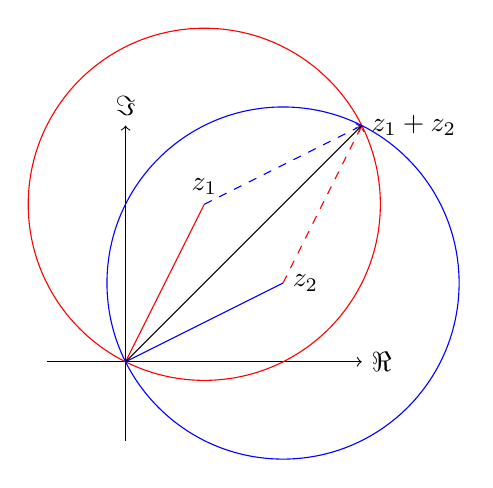
\begin{tikzpicture}
        \draw[->] (-1,0) -- (3,0) node[right] {$\Re$};
        \draw[->] (0,-1) -- (0,3) node[above] {$\Im$};
        \draw (0,0) -- (1,2) node[above] {$z_1$}[red];
        \draw (0,0) -- (2,1) node[right] {$z_2$}[blue];
        \draw (1,2) circle (2.2360679775)[red];
        \draw (2,1) circle (2.2360679775)[blue];
        \draw[dashed,->] (1,2) -- (3,3)[blue];
        \draw[dashed,->] (2,1) -- (3,3)[red];
        \draw (0,0) -- (3,3) node[right] {$z_1 + z_2$};
    \end{tikzpicture}
    \caption{Construction of $z_1 + z_2$}
    \label{Fig.2}
\end{figure}

\begin{corollary}[Subtraction of complex numbers]
    \label{cor:construction_sub}
    \lean{sub_M_Inf}
    \leanok
    \uses{def:set_of_constructable_points}
    For $z_1, z_2 \in M_{\infty}$ is $z_1 - z_2 \in M_{\infty}$.
\end{corollary}
\begin{proof}
    \uses{lem:construction_neg, lem:construction_add}
    By lemma \ref{lem:construction_neg} and \ref{lem:construction_add} we get $z_1 - z_2 = z_1 + (-z_2) \in M_{\infty}$.
\end{proof}

\begin{corollary}[Construction of parallel lines]
    \label{lem:construction_parallel_lines}
    \lean{parallel_lines_M_inf}
    \leanok
    \uses{def:set_of_constructable_points, def:set_of_lines, def:parallel}
    For $l \in \mathcal{L(M_{\infty})}$ and $z \in M_{\infty}$ is $\exists l' \in \mathcal{L(M_{\infty}): z\in l' \text{ and } l\|l'}$.
\end{corollary}
\begin{proof}
    \uses{def:line, def:set_of_lines, cor:construction_sub,lem:parallel_by_basis} 
    Let $l$ be a line through $x,y \in \mathcal{M_{\infty}}$ and $z \in \mathcal{M_{\infty}}$.\\
    After corollary \ref{cor:construction_sub} we get $z - x \in \mathcal{M_{\infty}}$ and therfore $z-x + y \in \mathcal{M_{\infty}}$\ref{lem:construction_add}.\\
    Define $l' = \{z, z-x+y\}$, then $l' \in \mathcal{L(M_{\infty})}$ and since a line is defined by two points and we moved them the same distence ($z-x$) $l'$ is parallel to $l$.\ref{lem:parallel_by_basis}
\end{proof}
%2.3.3
%TODO: Comper to mirrowed version
\begin{lemma}[Complex conjugation]
    \label{lem:construction_conj}
    \lean{conj_M_Inf}
    \leanok
    \uses{def:set_of_constructable_points}
    For $z \in M_{\infty}$ is $\overline{z} \in M_{\infty}$.
\end{lemma}
This constrution is teken from \cite{JAN_SCHRÖER:2023}.\\
Draw two crircles one with center $0$ and radius $\|z\|$ and a second with center $1$ and radius $\|z-1\|$ and take the intersection of the two circles.\ref{Fig.3}
\begin{proof}
    \uses{def:line, def:circle, lem:icc_M_inf, lem:M_in_M_inf}
    Define $c_1 = \{0,\dist 0 z\}$ and $c_2 = \{1,\dist 1 z\}$.\\
    By assumption $0, 1, z \in M_{\infty}$, so $c_1, c_2 \in \mathcal{C(M_{\infty})}$.\\
    \underline{Claim 1}: $\overline{z}$ is in $c_1$.
    \begin{proof}
        Unfolding the definition of $c_1:=\{x\in\mathbb{C} \mid\|x-0\|=\dist (0\ z)\}$.
        By the definition of the distence we get $\|0-\overline{z}\| = \|\overline{z}\| =\|z\| = \dist (0\ z)$.
    \end{proof}
    \underline{Claim 2}: $\overline{z}$ is in $c_2$.
    \begin{proof}
        Unfolding the definition of $c_2:=\{x\in\mathbb{C} \mid\|x-1\|=\dist (1\ z)\}$.
        By the definition of the distence we get $$\|1-\overline{z}\| = \|\overline{z}-1\| = \sqrt{(\Re(\overline{z})-1)^2 + \Im(\overline{z})^2} = \sqrt{(\Re(z)-1)^2 + \Im(z)^2} = \|z-1\|=\dist (1\ z).$$
    \end{proof}
    By claim 1 and 2 we get that $\overline{z} \in c_1 \cap c_2$. Futhermore  $\overline{z} $ is in $M_{\infty}$, after lemma \ref{lem:icc_M_inf}.
\end{proof}
\begin{figure}[h]
    \centering
    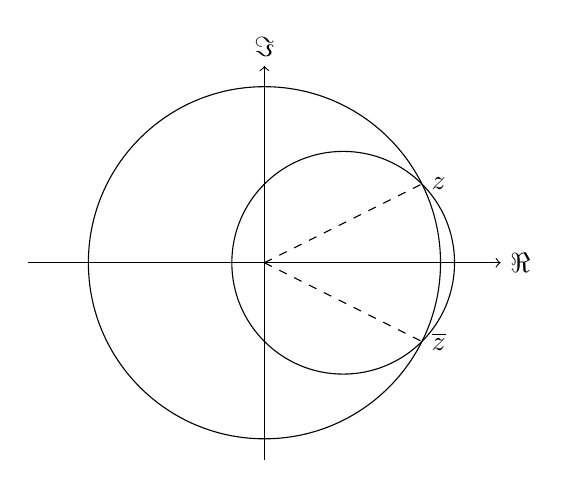
\begin{tikzpicture}
        \draw[->] (-3,0) -- (3,0) node[right] {$\Re$};
        \draw[->] (0,-2.5) -- (0,2.5) node[above] {$\Im$};
        \draw[dashed] (0,0) -- (2,1) node[right] {$z$};
        \draw[dashed] (0,0) -- (2,-1) node[right] {$\overline{z}$};
        \draw (0,0) circle (2.2360679775);
        \draw (1,0) circle (1.4142135624);
    \end{tikzpicture}
    \caption{Construction of $\overline{z}$}
    \label{Fig.3}
\end{figure}


\begin{lemma}[Construction $\imath r\in\mathcal{M}_{\infty}$ ]
    \label{lem:construction_imath_r}
    \lean{ir_M_inf}
    \leanok
    \uses{def:set_of_constructable_points}
    For $r \in \mathbb{R}\cap M_{\infty}$ is $\imath r \in M_{\infty}$.
\end{lemma}
First you need to construct the imaginary axis by drawing a line $l$ through two crircles with center $-1$ and $1$ and radius $2$. Then you can construct the point $\imath r$, by drawing a circle with center $0$ and radius $r$ and taking the intersection with the imaginary axis.\ref{Fig.4}
\begin{proof}
    \uses{def:line, def:circle, lem:construction_neg, lem:icc_M_inf, lem:ilc_M_inf, lem:M_in_M_inf}
    First we construct the imaginary axis. Define $c_1 = \{-1,2\}$ and $c_2 = \{1,2\}$.\\
    \underline{Claim 1}: $c_1, c_2 \in \mathcal{C(M_{\infty})}$
    \begin{proof}
        By assumption and lamma \ref{lem:construction_neg} we get $-1, 1 \in M_{\infty}$. Using $\dist(-1 1)=2$ we get $c_1, c_2 \in \mathcal{C(M_{\infty})}$, by the definition of the circle.
    \end{proof}
    \underline{Claim 2}: $\imath\sqrt{3}$ and $-\imath\sqrt{3}$ are in $c_1 \cap c_2$.
    \begin{proof}
        Unfolding the definition of $c_1:=\{x\in\mathbb{C} \mid\|x+1\|=2\}$ and $c_2:=\{x\in\mathbb{C} \mid\|x-1\|=2\}$.
        By the definition of the distence we get $\|-\imath\sqrt{3}+1\| = \sqrt{1 + 3} = 2$ and $\|\imath\sqrt{3}-1\| = \sqrt{1 + 3} = 2$.
    \end{proof}
    Now we define $l = \{\imath\sqrt{3}, -\imath\sqrt{3}\}$.\\
    \underline{Claim 3}: $l \in \mathcal{L(M_{\infty})}$
    \begin{proof}
        By claim 2 and \ref{lem:icc_M_inf} we get $\imath\sqrt{3}, -\imath\sqrt{3} \in M_{\infty}$, so $l \in \mathcal{L(M_{\infty})}$.
    \end{proof}
    To get $\imath r$ we define $c = \{0,|r|\}$.\\
    \underline{Claim 4}: $\imath r$ is in $c \cap l$.
    \begin{proof}
        It is clear that $\imath r \in c$. New using the definition of $l$ and $\lambda = \frac{r}{2\sqrt{3}+\frac{1}{2}}$ we get $(\frac{r}{2\sqrt{3}+\frac{r}{2}})\imath\sqrt{3} + (1-\frac{r}{2\sqrt{3}+\frac{r}{2}})(-\imath\sqrt{3}) = \imath r$. 
    \end{proof}
    Therfore $\imath r \in M_{\infty}$ after lemma \ref{lem:ilc_M_inf}.
\end{proof}
\begin{figure}[h]
    \centering
    \begin{tikzpicture}
        \tikzset{
            carc/.style args={#1:#2:#3}{
              insert path={+(#1:#3) arc (#1:#2:#3)}
            }
          }
          
        \draw[->] (-3,0) -- (3,0) node[right] {$\Re$};
        \draw[->] (0,-2.5) -- (0,2.5) node[above] {$\Im$};
        \coordinate[label=-45:$1$] (one) at (1,0);
        \coordinate[label=-135:$-1$] (mone) at (-1,0);
        \fill[black] (one) circle (2pt);
        \fill[black] (mone) circle (2pt);
        \draw[dashed] (one) [carc=110:250:2];
        \draw[dashed] (mone) [carc=70:-70:2];
        \coordinate[label=45:$r$] (r) at (2,0);
        \coordinate[label=135:$\imath r$] (ir) at (0,2);
        \fill[black] (r) circle (2pt);
        \fill[black] (ir) circle (2pt);
        \draw (0,0) [carc=-10:100:2];
    \end{tikzpicture}
    \caption{Construction of $\imath r$}
    \label{Fig.4}
\end{figure}

\begin{corollary}[Construction of $\imath$]
    \label{cor:construction_imath}
    \lean{imath_M_inf}
    \leanok
    \uses{def:set_of_constructable_points}
    $\imath \in M_{\infty}$.
\end{corollary}
\begin{proof}
    \uses{lem:construction_imath_r, lem:M_in_M_inf}
    By lemma \ref{lem:construction_imath_r} with $r = 1$ and the definition of $\mathcal{M}$ we get $\imath \in M_{\infty}$.
\end{proof}

\begin{lemma}[Construction of real part]
    \label{lem:construction_real}
    \lean{real_in_M_inf}
    \leanok
    \uses{def:set_of_constructable_points}
    For $z \in M_{\infty}$ is $z.re \in M_{\infty}$.
\end{lemma}
\begin{proof}
    \uses{cor:construction_sub}
    Without loss of generality we can assume that $z \in \C\setminus\R$.\\
    Define the lines $l = \{z, \overline{z}\}$ and $l_{\Re} = \{1, 0\}$.\\
    Using Lemma \ref{lem:construction_conj}, they are in $\mathcal{L(M_{\infty})}$, by the normal argumentation.\\
    To show that $z.re \in l \cap l_{\Re}$ we use $t:= 1/2$ for $l$ and $t:= z.re$ for $l_{\Re}$.
\end{proof}
\begin{lemma}[Construction of imaginary part]
    \label{lem:construction_imag}
    \lean{im_in_M_inf}
    \leanok
    \uses{def:set_of_constructable_points}
    For $z \in M_{\infty}$ is $z.im \in M_{\infty}$.
\end{lemma}

\begin{lemma}[Multiplication of positve real numbers]
    \label{lem:construction_mul}
    \lean{ab_in_M_inf}
    \leanok
    \uses{def:set_of_constructable_points}
    For $a, b \in M_{\infty}\cap\R$ is $a \cdot b \in M_{\infty}$.
\end{lemma}
This constrution is taken from \cite{cox2012galois}.\\
To get the point $a\cdot b$ we draw a line trough $a$ and $\imath$ and a parallel line through $\imath b$. The intersection of the second line with the real axis is $a\cdot b$.\ref{Fig.5} 
\begin{proof}
    \uses{def:line, def:set_of_lines, lem:ill_M_inf, lem:construction_imath_r, cor:construction_imath, lem:construction_add, cor:construction_sub}
    Define the three lines $l = \{a+\imath b - \imath, \imath b\}$ and $l_{\Re} = \{1,0\}$.\\
    \underline{Claim 1}: $l \in \mathcal{L(M_{\infty})}$
    \begin{proof}
        By assumption is $b \in M_{\infty}$ so after Lemma \ref{lem:construction_imath_r} $\imath b \in M_{\infty}$. Futhermore $l_2 \in \mathcal{L(M_{\infty})}$ after Claim 1 and Lemma \ref{lem:construction_parallel_lines}.
    \end{proof}
    \underline{Claim 2}: $l_{\Re} \in \mathcal{L(M_{\infty})}$
    \begin{proof}
        By assumption $0, 1 \in M_{\infty}$, so $l_{\Re} \in \mathcal{L(M_{\infty})}$.
    \end{proof}
    To show that $a\cdot b \in M_{\infty}$ we need to show that $l \cap l_{\Re} \in M_{\infty}$\ref{lem:ill_M_inf}. That $ab \in l_{\Re} \cap l$ is clear after definition $t=ab$. For $ab \in l$ we use $t=b$ and get $t(a+\imath b - \imath) + (1-t)\imath b  \stackrel{t:=b}{=}ba + \imath b^2 -\imath b + \imath b -\imath b^2 = a\cdot b$.
\end{proof}
\begin{remark}
    This construction uses parallel lines, but it is not needed for the proof of the lemma.
\end{remark}
\begin{figure}
    \centering
    \begin{tikzpicture}
        \draw[->] (-0.5,0) -- (5,0) node[right] {$\Re$};
        \draw[->] (0,-0.5) -- (0,3) node[above] {$\Im$};
        \coordinate[label=135:$\imath$] (i) at (0,1);
        \coordinate[label=-90:$a$] (a) at (2,0);
        \coordinate[label=135:$\imath b$] (ib) at (0,2);
        \coordinate[label=-90:$ab$] (ab) at (4,0);
        \fill[black] (i) circle (2pt);
        \fill[black] (a) circle (2pt);
        \fill[black] (ib) circle (2pt);
        \fill[black] (ab) circle (2pt);
        \draw (a) -- (i);
        \draw (ib) -- (ab);
    \end{tikzpicture}
    \caption{Construction of $z_1 \cdot z_2$}
    \label{Fig.5}
\end{figure}

\begin{corollary}[Multiplication of complex numbers]
    \label{cor:construction_mul_complex}
    %\lean{mul_in_M_inf}
    %\leanok
    \uses{def:set_of_constructable_points}
    For $z_1, z_2 \in M_{\infty}$ is $z_1 \cdot z_2$ in $M_{\infty}$.
\end{corollary}
\begin{proof}
    \uses{lem:construction_mul, lem:construction_add, cor:construction_sub}
    Let $z_1 = a + \imath b$ and $z_2 = c + \imath d$. Then $$z_1 \cdot z_2 = (a + \imath b) \cdot (c + \imath d) = (a \cdot c - b \cdot d) + \imath (a \cdot d + b \cdot c).$$
    
\end{proof}

\begin{lemma}[Invers of a pos real number]
    \label{lem:construction_inv}
    \lean{ainv_in_M_inf}
    \leanok
    \uses{def:set_of_constructable_points}
    If $a \in M_{\infty}\cap\R$, then $a^{-1}$ is in  $M_{\infty}$.
\end{lemma}

This can be construceted analog to the multiplication of positve real numbers. Usind the fact that $a\cdot a^{-1} = 1$. Draw a line through $1$ and $\imath a$ and a parallel line through $\imath$. The intersection of the second line with the real axis is $a^{-1}$.\ref{Fig.6}
\begin{proof}
    \uses{def:line, def:set_of_lines, lem:ill_M_inf, lem:construction_imath_r, cor:construction_imath, lem:construction_add, cor:construction_sub}
    The proof is analog to the proof of Lemma \ref{lem:construction_mul} we just need two lines $l = \{1-\imath z + \imath, \imath\}$ and $l_{\Re} = \{1,0\}$.\\
    With  out loss of generality we can assume that $a \ne 0$.\\
    That there are in $\mathcal{L(M_{\infty})}$ follows analog to the proof of Lemma \ref{lem:construction_mul}.\\ 
    So we have just to show that $z^{-1} \in l$, i.e. $\exists t: t  (1 - \imath a + \imath) + (1 - t)  I = a^{-1}$ $$t  (1 - \imath a + \imath) + (1 - t)  \imath \stackrel{t:=a^{-1}}{=}  a^{-1} - a^{-1} \imath a + a^{-1}\imath + \imath - a^{-1}\imath = a^{-1}.$$
    The rest follws analog.
\end{proof}
\begin{figure}
    \centering
    \begin{tikzpicture}
        \draw[->] (-1,0) -- (2,0) node[right] {$\Re$};
        \draw[->] (0,-1) -- (0,3) node[above] {$\Im$};
        \coordinate[label=135:$\imath$] (i) at (0,1);
        \coordinate[label=-90:$1$] (1) at (1,0);
        \coordinate[label=135:$\imath a$] (ia) at (0,2);
        \coordinate[label=-90:$a^{-1}$] (ainv) at (0.5,0);
        \fill[black] (i) circle (2pt);
        \fill[black] (1) circle (2pt);
        \fill[black] (ia) circle (2pt);
        \fill[black] (ainv) circle (2pt);
        \draw (1) -- (ia);
        \draw (i) -- (ainv);
    \end{tikzpicture}
    \caption{Construction of $z^{-1}$}
    \label{Fig.6}
\end{figure}